% !TEX encoding = UTF-8 Unicode

\documentclass[a4paper, 12pt]{article}

\usepackage[T2A]{fontenc}
\usepackage[utf8x,utf8]{inputenc}
\usepackage[serbian]{babel}
%\usepackage[english,serbianc]{babel}
\usepackage{amssymb}
\usepackage{amsmath}

\usepackage{color}
\usepackage{url}
\usepackage[unicode]{hyperref}
\hypersetup{colorlinks,citecolor=green,filecolor=green,linkcolor=blue,urlcolor=blue}
\usepackage{graphicx}
\graphicspath{ {./slike/} }

\begin{document}

\title{Slobodna bacanja}

\author{Matija Miličević, Jovana Rađenović}

\maketitle

\section{Zadatak}

Košarkaš prilikom slobodnog bacanja izbacuje loptu sa visine koja odgovara 5/4 sopstvene visine. Ako zanemarimo trenje vazduha, i ako je ugao bacanja $\theta$, da bi lopte prošle centrom obruča potrebna je brzina izbačaja $v_\theta$. Sa istom brzinom $v_\theta$ lopta će ući u koš i za bliske uglove $[\theta_1, \theta_2]$ (a da ne dodirne obruč). Za zadatu visinu košarkaša h odrediti onaj ugao bacanja $\theta$ koji obezbeđuje maksimalnu toleranciju $\theta_2 - \theta_1$. Rezultate tabelirati za omiljeni košarkaški klub ili reprezentaciju.

\section{Pojmovi}

Osnovni pojmovi:\\
$h$ - visina košarkaša koji izvodi slobodna bacanja;\\
$h_k$ - visina koša;\\
$\theta$ - ugao izbačaja;\\
$v_\theta$ - brzina izbačaja za ugao $\theta$ pri kojoj lopta prolazi kroz centar obruča;\\
$d_c$ - rastojanje od košarkaša (y-ose) do centra obruča;\\
$r_l$ - poluprečnik lopte;\\
$r_o$ - poluprečnik obruča;\\

%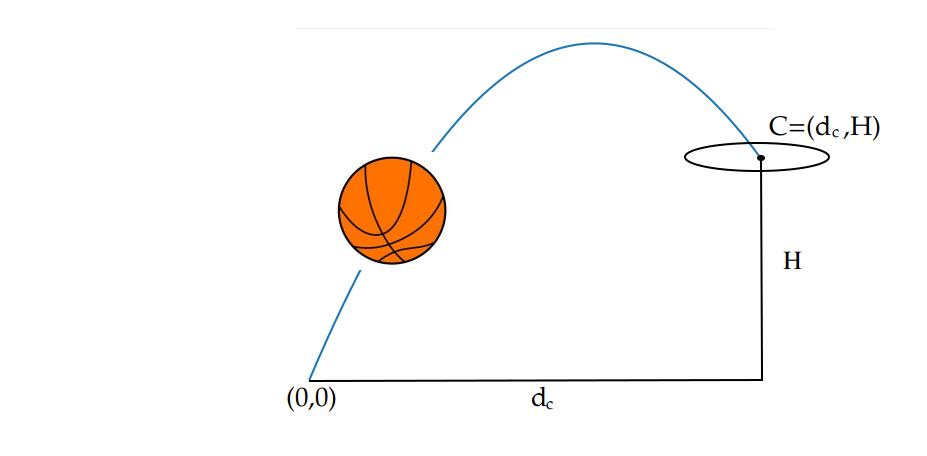
\includegraphics[width=7cm, height=4cm]{pic1} %TODO

\pagebreak


\section{Postavka} %TODO

Podrazumevaćemo:
\begin{itemize}

\item da je poluprečnik lopte $r_l$ manji od poluprečnika obruča $r_o$:
\[r_l<r_o\] %(3.1.1)

\item da je $\theta$ između $0^0$ i $90^0$:\\
\[0 < \theta < \pi/2\]

\item da je visina koša $h_k$ veća od visine izbačaja košarkaša $\dfrac{_5}{^4}h$:\\
\[h_k > \dfrac{_5}{^4}h\]  %\hfill \centerline{}
%(ovo nije obavezno ali olakšava crtanje slike)\\

\end{itemize}


Posmatraćemo centar lopte kao materijalnu tačku $(x,y)$ koja počinje svoj put iz tačke $(x_0,y_0) = (0,\dfrac{_5}{^4}h)$. Da bi lopta prošla kroz centar obruča u jednom trenutku mora važiti $(x,y) = C$, gde je $C = (d_c,h_k)$.\\

Pošto su visina koša i košarkaša konstantne veličine možemo da transliramo ceo sistem tako da početna tačka centra lopte bude $(x_0,y_0) = (0,0)$, a tačka centra obruča $C = (d_c,h_k-\dfrac{_5}{^4}h)$.
Zbog jednostavnosti zapisa uzećemo da je $H = h_k-\dfrac{_5}{^4}h$, odnosno $C = (d_c,H)$.\\


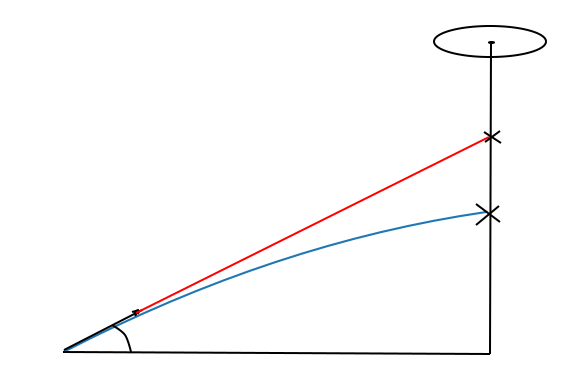
\includegraphics[width=10cm, height=5cm]{pic2} %TODO sredi + naznačiti $y_{max}$)\\

Po ovoj slici možemo primetiti da je polazni problem u stvari jedna vrsta problema kosog hica.

\pagebreak

\subsection{Kretnja lopte}

Možemo da vidimo da na $x$ koordinatu lopte ne utiče nijedna sila (otpor vazduha zanemarujemo), a pošto se lopta kreće brzinom zadatom pri šutu dolazimo da zaključka da važi:\\

\[x(t) = x_0 + v_{\theta x}\cdot t\]

Gde su: $x_0 = 0$; $v_{\theta x} = v_\theta \cdot \cos \theta$; odnosno:

\[x(t) = v_\theta \cdot \cos \theta \cdot t\]

Sa druge strane na $y$ koordinatu sve vreme utiče gravitacija. Uz početnu brzinu zadatu šutom možemo da zaključimo da važi:

\[y(t) = y_0 + v_{\theta y} \cdot t - \dfrac{g \cdot t^2}{2}\]

gde je $g \approx 9.81\dfrac{_m}{^{s^2}}$. Pošto važi da su: $y_0 = 0$; $v_{\theta y} = v_\theta \cdot \sin \theta$; sledi:

\[y(t) = v_{\theta} \cdot \sin \theta\cdot t - \dfrac{g}{2} \cdot t^2\]

Dakle, koordinate centra lopte u svakom trenutku su opisane jednačinama:

\[x(t) = v_\theta \cdot \cos \theta \cdot t\]

\[y(t) = v_{\theta} \cdot \sin \theta \cdot t - \dfrac{g}{2} \cdot t^2\]

\subsection{Uslovi za prolazak lopte kroz obruč}

Da bi lopta prošla kroz obruč ona mora prvo da prebaci visinu obruča. Mi utičemo na ugao šuta.

\section{Model: dvostruka iteracija}

\end{document}